% ============================================================
% 7. USE CASES
% This file is included from main.tex under Section 7.
% Do NOT use \section{} here.
% ============================================================

\subsection{Overview}

The Use Case Analysis identifies the major functional interactions between
the Dikaios Amanah system and its three primary stakeholder groups:
Business Owner, Retail Investor, and System Administrator.

The use cases are derived from the functional scope of the proposed system,
which includes user authentication, business verification, document
management, investment campaign management, investment tracking, portfolio
management, profit declaration, notifications, activity logging, and the
Permissioned Trust and Audit Layer. These functions support the proposed
objective of connecting verified businesses with verified retail investors
through a transparent Musharakah-based investment process.

\subsection{Primary Actors}

The Dikaios Amanah system has three primary actors.

\begin{itemize}
    \item \textbf{Business Owner:} Registers a business, provides business
    information, uploads verification documents, submits verification
    requests, creates investment campaigns, monitors campaigns, and declares
    business profits.

    \item \textbf{Retail Investor:} Registers and completes the required
    verification process, browses verified businesses and investment
    campaigns, participates in investment opportunities, and monitors
    investment and portfolio information.

    \item \textbf{System Administrator:} Manages users, reviews business
    verification requests, validates submitted information, approves or
    rejects businesses, monitors system activities, and reviews audit records.
\end{itemize}


% ============================================================
% USE CASE DIAGRAM
% ============================================================

\subsection{Use Case Diagram}

The Use Case Diagram presents the major functional interactions between the
three primary actors and the Dikaios Amanah system.

\begin{figure}[H]
    \centering
    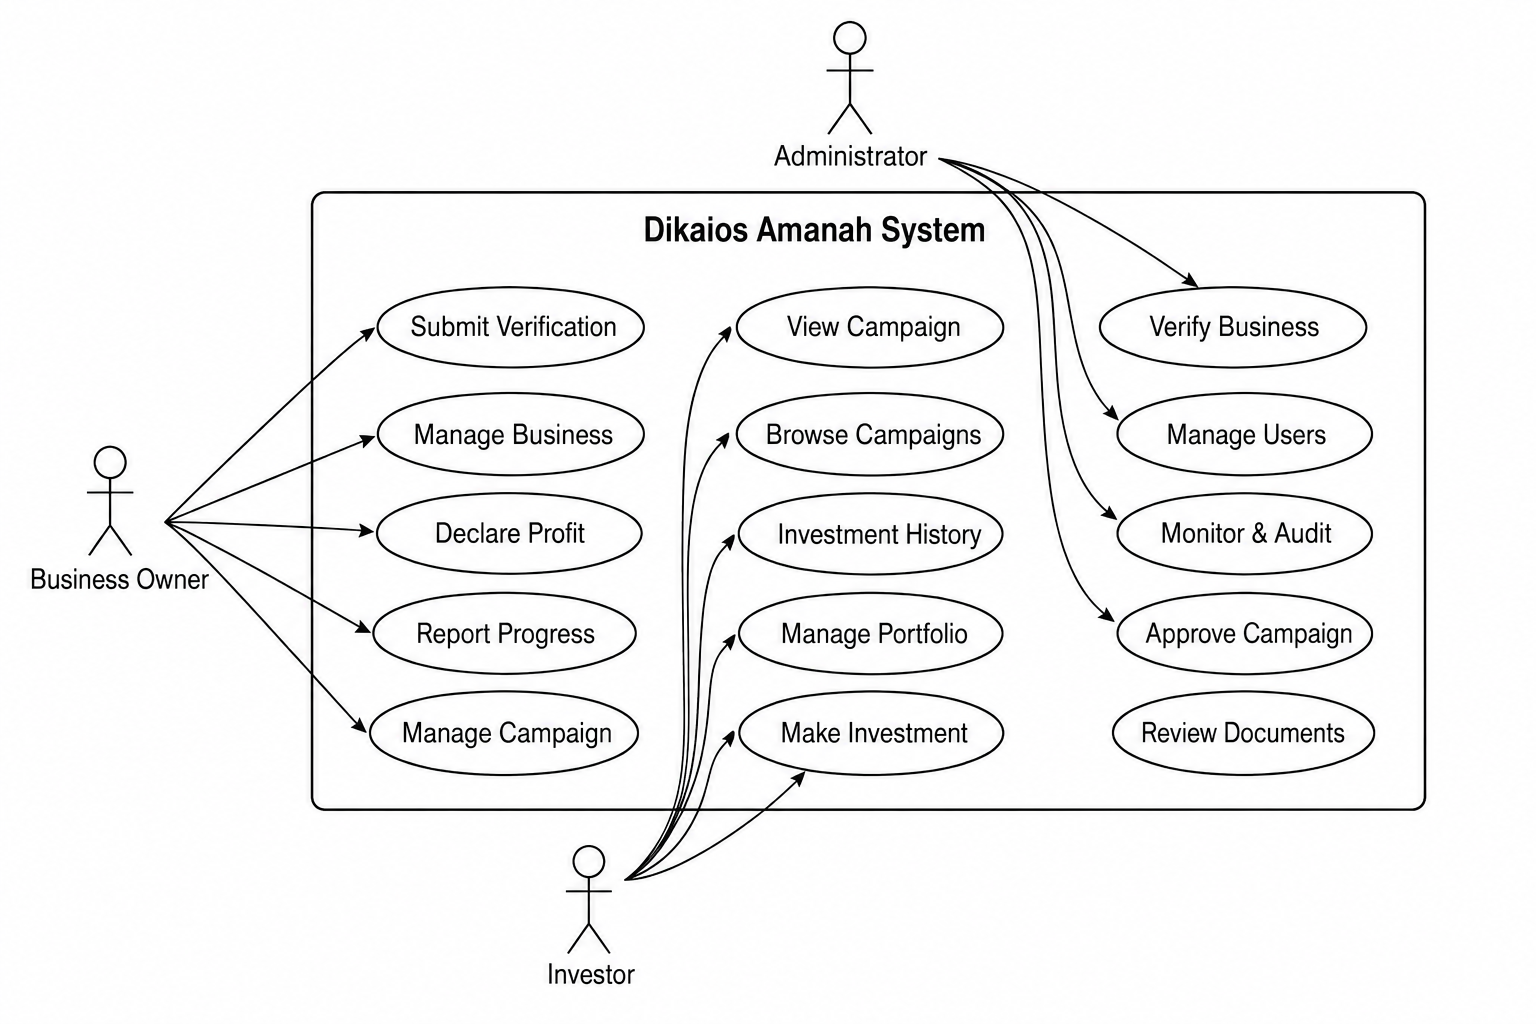
\includegraphics[width=\textwidth]{images/use_case.png}
    \caption{Dikaios Amanah Use Case Diagram}
    \label{fig:use-case}
\end{figure}


% ============================================================
% BUSINESS OWNER USE CASES
% ============================================================

\subsection{Business Owner Use Cases}

The Business Owner interacts with the system primarily to establish a
verified business profile and obtain investment through Musharakah-based
campaigns.

\subsubsection{Register and Authenticate}

The Business Owner creates an account and authenticates using the secure
authentication mechanism provided by the system.

\textbf{Precondition:}
The user does not already have an active account.

\textbf{Main Flow:}
\begin{enumerate}
    \item The Business Owner provides registration information.
    \item The system validates the submitted information.
    \item The system creates the user account.
    \item The Business Owner logs into the system.
    \item The system authenticates the credentials and provides access to the
    Business Owner dashboard.
\end{enumerate}

\textbf{Postcondition:}
The Business Owner is authenticated and can access authorized system
functions.


\subsubsection{Submit Business Verification}

The Business Owner submits business information and supporting documents for
administrative verification.

\textbf{Precondition:}
The Business Owner is authenticated.

\textbf{Main Flow:}
\begin{enumerate}
    \item The Business Owner enters business information.
    \item The Business Owner uploads the required documents.
    \item The system validates the submitted information.
    \item The system stores the verification record and documents.
    \item The system notifies the Administrator.
\end{enumerate}

\textbf{Postcondition:}
The business verification request is available for Administrator review.


\subsubsection{Create Investment Campaign}

A verified Business Owner creates an investment campaign containing the
required business and funding information.

\textbf{Precondition:}
The Business Owner and business have been verified.

\textbf{Main Flow:}
\begin{enumerate}
    \item The Business Owner selects the campaign creation function.
    \item The Business Owner provides campaign title and description.
    \item The Business Owner specifies the funding goal and related
    information.
    \item The system validates the information.
    \item The system creates the campaign.
\end{enumerate}

\textbf{Postcondition:}
The campaign is stored and can be made available to eligible investors.


\subsubsection{Monitor Investment Campaign}

The Business Owner monitors campaign status and funding progress.

\textbf{Main Flow:}
\begin{enumerate}
    \item The Business Owner opens the campaign dashboard.
    \item The system retrieves campaign information.
    \item The system displays current funding and campaign status.
\end{enumerate}


\subsubsection{Declare Profit}

The Business Owner submits profit information associated with an investment
campaign.

\textbf{Precondition:}
An applicable investment campaign exists.

\textbf{Main Flow:}
\begin{enumerate}
    \item The Business Owner selects the profit declaration function.
    \item The Business Owner enters the profit amount and reporting period.
    \item The system validates the submitted information.
    \item The system stores the profit declaration.
    \item The event is recorded in the audit layer.
\end{enumerate}

\textbf{Postcondition:}
The profit declaration is stored and available for authorized processing
and monitoring.


% ============================================================
% INVESTOR USE CASES
% ============================================================

\subsection{Retail Investor Use Cases}

Retail Investors interact with the system to discover verified investment
opportunities, participate in campaigns, and monitor their investments.

\subsubsection{Register and Complete Investor Verification}

The Retail Investor creates an account and provides the required information
for verification.

\textbf{Main Flow:}
\begin{enumerate}
    \item The Investor registers an account.
    \item The system validates the submitted information.
    \item The Investor provides required verification information.
    \item The system stores the verification information.
    \item The Administrator reviews the submitted information.
\end{enumerate}

\textbf{Postcondition:}
The Investor account is available according to its verification status.


\subsubsection{Browse Verified Businesses}

The Investor searches and views verified businesses available on the
platform.

\textbf{Main Flow:}
\begin{enumerate}
    \item The Investor opens the investment marketplace.
    \item The system retrieves eligible verified businesses.
    \item The system displays business profiles and available campaigns.
    \item The Investor selects a business or campaign for further review.
\end{enumerate}


\subsubsection{Review Investment Campaign}

The Investor reviews the information associated with an investment
opportunity before making an investment decision.

The system provides relevant campaign information, business information,
funding progress, and available investment details.


\subsubsection{Participate in Investment Campaign}

The Investor participates in an available Musharakah-based investment
campaign.

\textbf{Precondition:}
The Investor is authenticated and eligible to participate.

\textbf{Main Flow:}
\begin{enumerate}
    \item The Investor selects an available campaign.
    \item The Investor enters the intended investment amount.
    \item The system validates the investment information.
    \item The system records the investment.
    \item The investment status is updated.
    \item The event is recorded in the audit layer.
\end{enumerate}

\textbf{Postcondition:}
The investment appears in the Investor's portfolio.


\subsubsection{Monitor Investment Portfolio}

The Investor monitors investment status and portfolio information.

\begin{enumerate}
    \item The Investor opens the portfolio dashboard.
    \item The system retrieves investment records.
    \item The system displays investment status and relevant portfolio
    information.
\end{enumerate}


% ============================================================
% ADMINISTRATOR USE CASES
% ============================================================

\subsection{Administrator Use Cases}

The Administrator is responsible for verification, approval, monitoring,
and administrative control of the platform.

\subsubsection{Review Business Verification}

The Administrator reviews submitted business verification requests.

\textbf{Main Flow:}
\begin{enumerate}
    \item The Administrator opens the pending verification list.
    \item The system retrieves the submitted verification information.
    \item The Administrator reviews business information and documents.
    \item The Administrator approves or rejects the verification request.
    \item The system updates the verification status.
    \item The system records the decision in the audit layer.
    \item The Business Owner is notified of the result.
\end{enumerate}


\subsubsection{Manage Users}

The Administrator manages authorized users and their system status.

Possible administrative actions include reviewing user information,
updating account status, and managing access according to the user's role.


\subsubsection{Monitor System Activity}

The Administrator reviews system activity and important operational events.

The system provides activity records generated by important actions such as
verification decisions, investment activities, and other critical operations.


\subsubsection{Review Audit Records}

The Administrator reviews audit records generated by the Permissioned Trust
and Audit Layer.

Audit records provide tamper-evident evidence of important system events and
support accountability and transparency.


% ============================================================
% USE CASE SUMMARY
% ============================================================

\subsection{Use Case Summary}

\begin{table}[H]
\centering
\caption{Dikaios Amanah Use Case Summary}
\label{tab:use-case-summary}
\begin{tabularx}{\textwidth}{>{\raggedright\arraybackslash}p{0.22\textwidth}
>{\raggedright\arraybackslash}p{0.22\textwidth}
X}
\toprule
\textbf{Actor} & \textbf{Use Case} & \textbf{Description} \\
\midrule

Business Owner &
Register and Authenticate &
Creates an account and securely accesses the platform. \\

Business Owner &
Submit Business Verification &
Submits business information and supporting documents for verification. \\

Business Owner &
Create Investment Campaign &
Creates a Musharakah-based investment campaign. \\

Business Owner &
Monitor Campaign &
Monitors campaign status and funding progress. \\

Business Owner &
Declare Profit &
Submits profit information for an investment campaign. \\

Retail Investor &
Register and Verify &
Creates an account and completes required verification. \\

Retail Investor &
Browse Businesses &
Views verified businesses and available opportunities. \\

Retail Investor &
Review Campaign &
Examines investment campaign information before investing. \\

Retail Investor &
Participate in Investment &
Records participation in an eligible investment campaign. \\

Retail Investor &
Monitor Portfolio &
Views investment status and portfolio information. \\

Administrator &
Review Verification &
Reviews business information and supporting documents. \\

Administrator &
Manage Users &
Manages user accounts and access status. \\

Administrator &
Monitor Activity &
Reviews important platform activities. \\

Administrator &
Review Audit Records &
Reviews tamper-evident records of critical system events. \\

\bottomrule
\end{tabularx}
\end{table}


% ============================================================
% SEQUENCE DIAGRAM
% ============================================================

\subsection{Business Verification Sequence}

The sequence diagram describes the interaction between the Business Owner,
Administrator, web interface, backend API, verification service, database,
audit service, and notification service during business verification.

\begin{figure}[H]
    \centering
    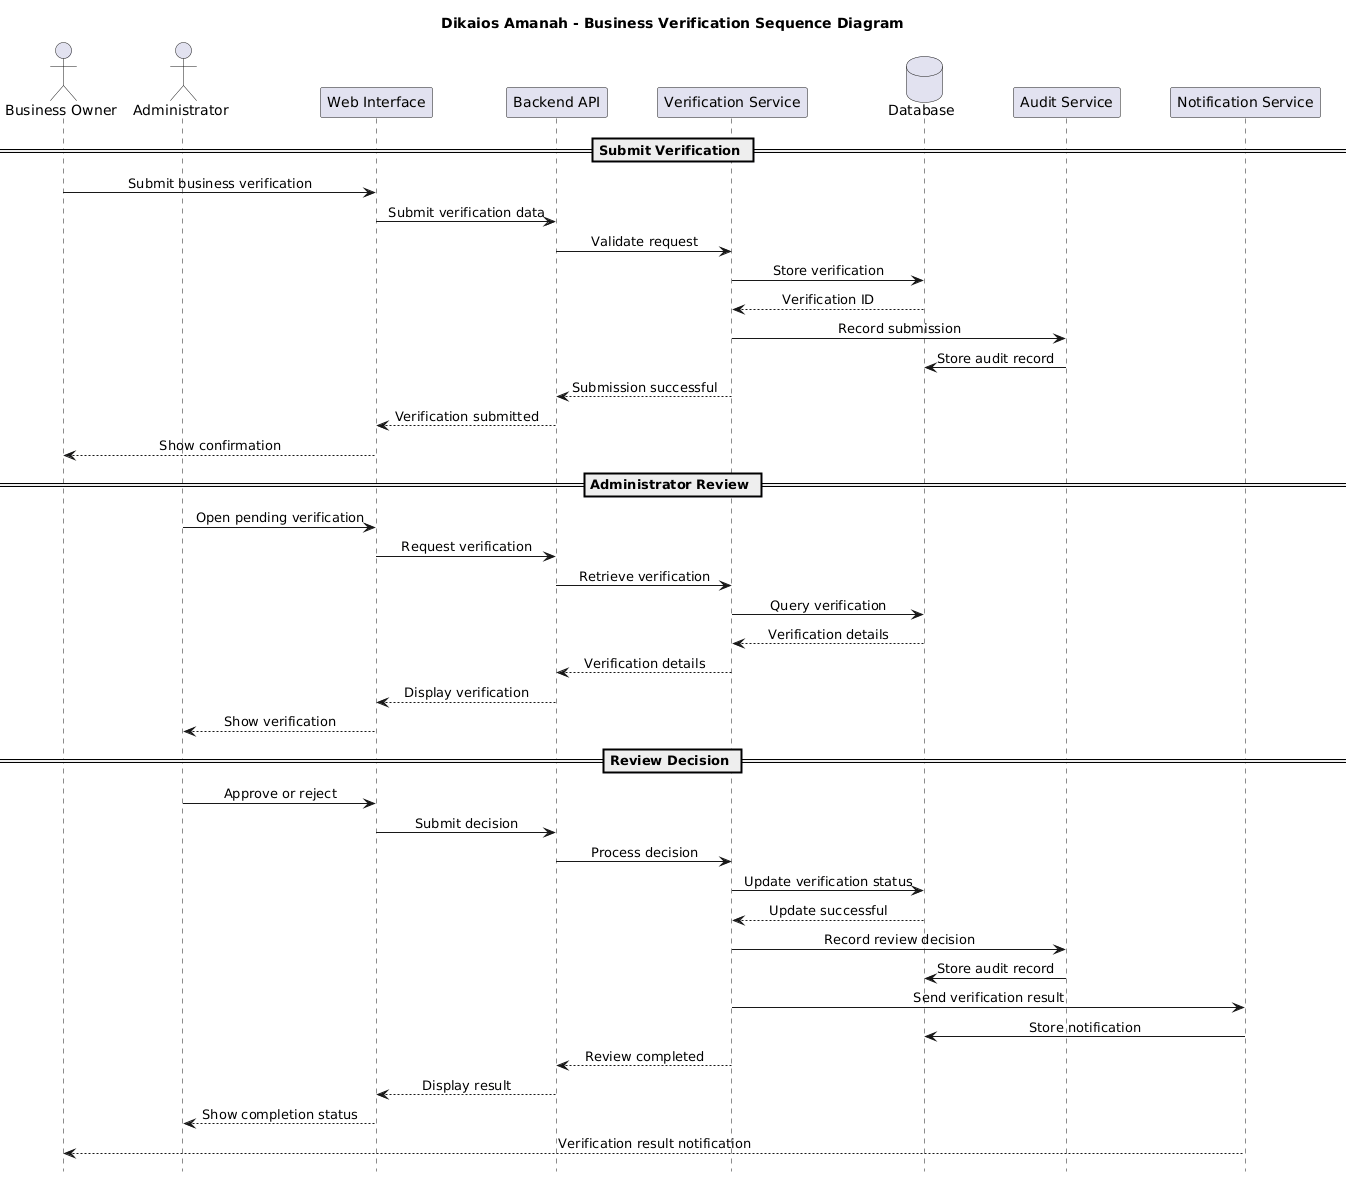
\includegraphics[width=\textwidth]{images/sequence_diagram.png}
    \caption{Business Verification Sequence Diagram}
    \label{fig:sequence-diagram}
\end{figure}


% ============================================================
% ACTIVITY DIAGRAM
% ============================================================

\subsection{Business Verification Activity}

The activity diagram illustrates the workflow beginning with business
information submission and continuing through validation, administrative
review, approval or rejection, and notification.

\begin{figure}[H]
    \centering
    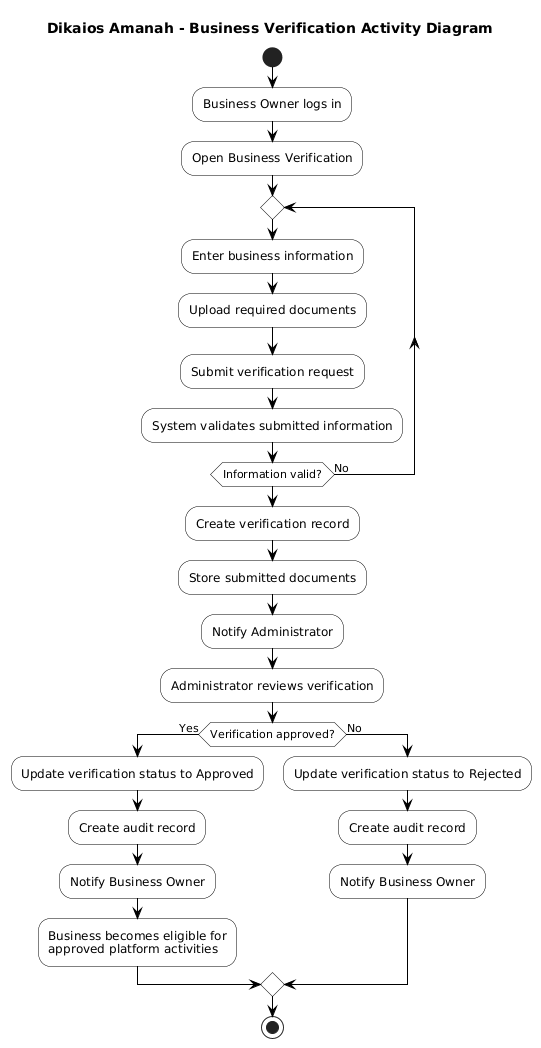
\includegraphics[width=0.85\textwidth]{images/activity_diagram.png}
    \caption{Business Verification Activity Diagram}
    \label{fig:activity-diagram}
\end{figure}


% ============================================================
% CLASS DIAGRAM
% ============================================================

\subsection{System Class Structure}

The class diagram presents the principal entities involved in the Dikaios
Amanah system, including users, business owners, administrators, businesses,
campaigns, investments, verifications, documents, profit declarations,
notifications, and audit records.

\begin{figure}[H]
    \centering
    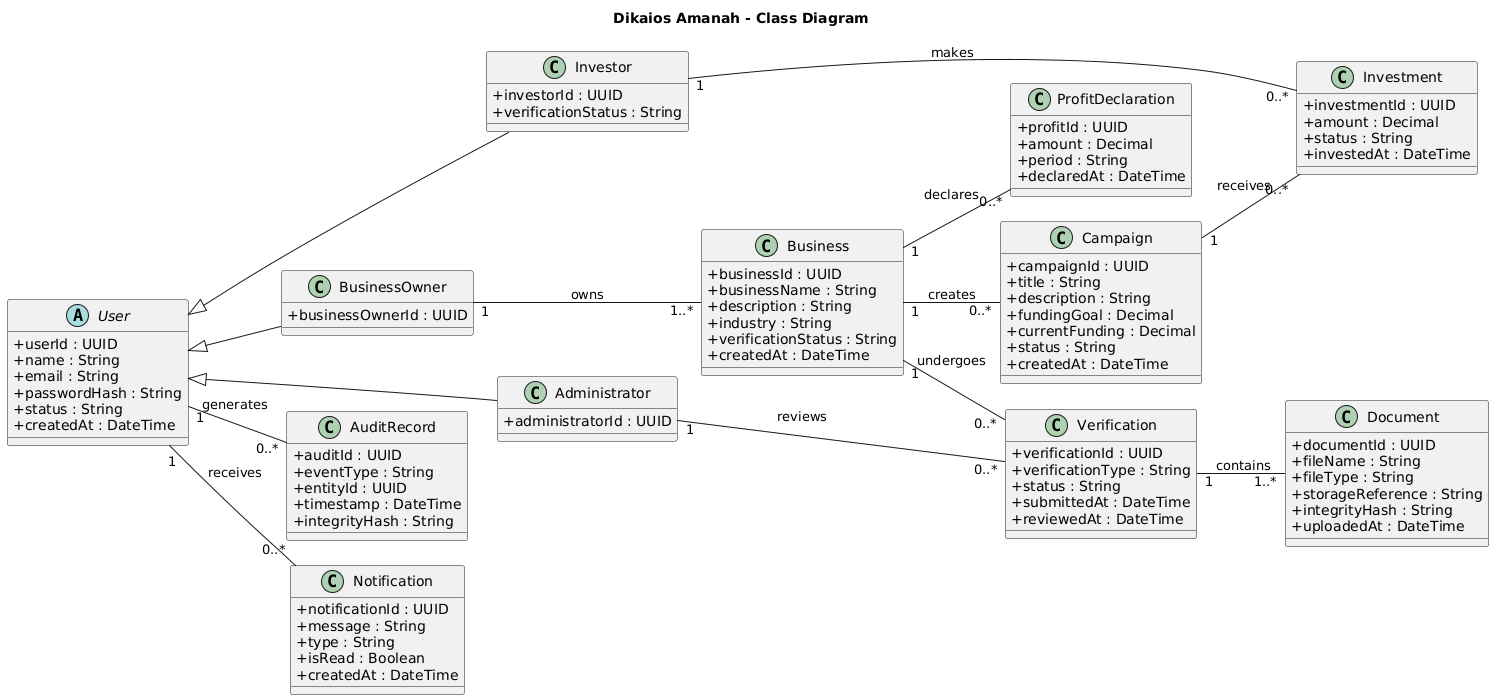
\includegraphics[width=\textwidth]{images/class_diagram.png}
    \caption{Dikaios Amanah Class Diagram}
    \label{fig:class-diagram}
\end{figure}


% ============================================================
% COMPONENT DIAGRAM
% ============================================================

\subsection{System Component Structure}

The component diagram presents the major software components of the proposed
Dikaios Amanah architecture and their relationships with the application
database and document storage.

\begin{figure}[H]
    \centering
    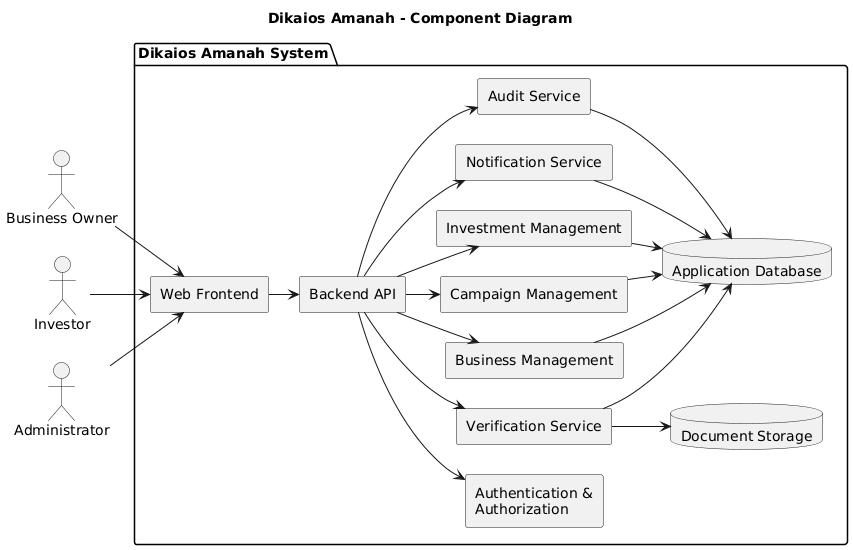
\includegraphics[width=\textwidth]{images/component_diagram.png}
    \caption{Dikaios Amanah Component Diagram}
    \label{fig:component-diagram}
\end{figure}


% ============================================================
% FISHBONE / ISHIKAWA DIAGRAM
% ============================================================

\subsection{Problem Cause Analysis}

The Fishbone (Ishikawa) Diagram identifies the major causes contributing to
the central problem of lack of trust and transparency in small-business
investment.

The identified cause categories include Information, Verification,
Transparency, Security, Process, and Investor Awareness.

\begin{figure}[H]
    \centering
    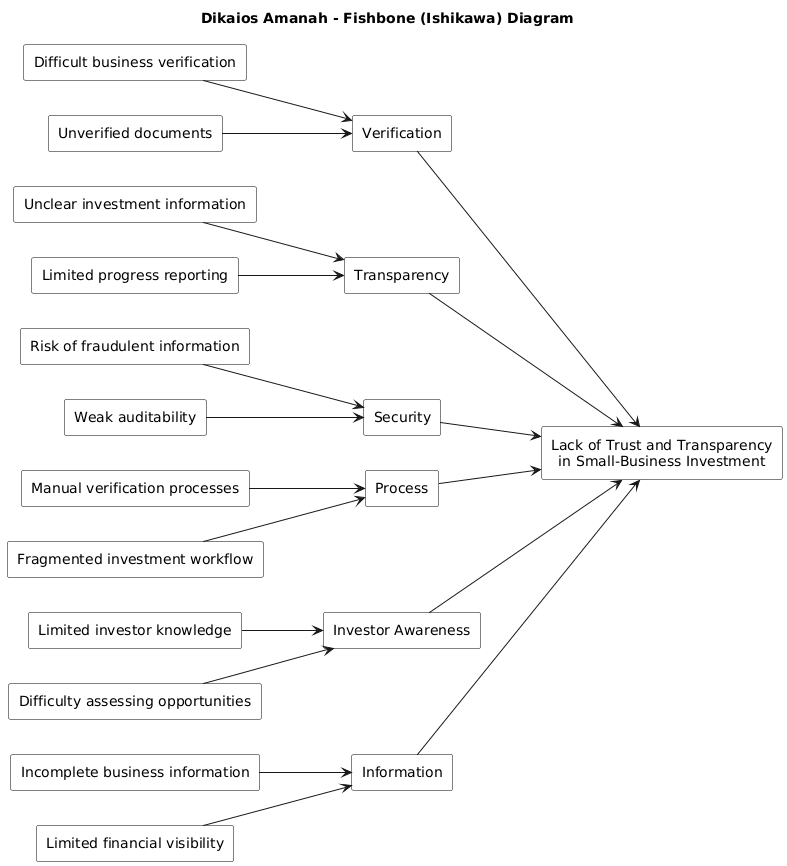
\includegraphics[width=\textwidth]{images/fishbone_diagram.png}
    \caption{Dikaios Amanah Fishbone (Ishikawa) Diagram}
    \label{fig:fishbone-diagram}
\end{figure}


% ============================================================
% RELATIONSHIP TO SYSTEM REQUIREMENTS
% ============================================================

\subsection{Relationship to System Requirements}

The identified use cases provide the functional foundation for subsequent
requirements specification and system design. They identify the primary
interactions that must be supported by the system and provide a basis for
deriving functional requirements, database entities, system workflows, and
software components.

The proposed system scope includes user authentication, business
verification, secure document management, investment campaign creation,
campaign browsing, investment tracking, portfolio management, profit
declaration, notifications, activity logging, and the Permissioned Trust
and Audit Layer.
